	\documentclass[12pt,a4paper]{article}
\usepackage[utf8]{inputenc}
\usepackage{amsmath}
\usepackage{amsfonts}
\usepackage{amssymb}
\usepackage{graphicx}
\usepackage{setspace}
\usepackage{nicefrac}
\usepackage{bbold}
\usepackage{booktabs} % toprule, midrule, ..
\usepackage[left=2.00cm, right=2.00cm, top=2.00cm, bottom=2.00cm]{geometry}
\usepackage{siunitx}
\usepackage{url}
\usepackage{paralist}
\usepackage{enumitem} % special labels
\usepackage{multirow}
\usepackage{rotating}

\usepackage{minted}

\usepackage{longtable,tabu}

\usepackage{multicol,multirow}
\usepackage{tikz}

\usepackage{hhline}
\usepackage{placeins}

\usetikzlibrary{shapes,snakes,trees}

\definecolor{mintedbg}{rgb}{.97,.97,1.}
\setminted{breaklines,bgcolor=mintedbg}

\title{Project: Bubble Bobble\\Phase 3}
\author{Pierre Beaujean}
\date{Due for May 6$^\text{th}$, 2018}

\setlength{\jot}{10pt} % aligns
\renewcommand{\arraystretch}{1.1}
\setlength{\tabcolsep}{0.20cm}
\onehalfspacing

\begin{document}
\maketitle

\section{Introduction}

Bubble Booble, released in 1986 by Taito in arcades, is an action platformer type video game where the player controls two dragons, named Bub (green) and Bob (blue). To save their girlfriends, kidnapped in the last stage of the game, the dragons must go through different levels by blowing bubbles to trap their enemies, then burst them. When they do, they create items that, if collected, give them a certain amount of point. If there is no more monsters to trap, the dragons go to the next one after a given amount of time (or if all the items have been collected). One level is limited to a single screen, constituted of platforms (and walls in the left and the right of the screen). The dragons can move along the platform, jump over higher ones and fall to lower ones. Note that if the dragon fall into a gap in the bottom of the screen, it reappears on the top. Monsters chase the dragons, which loses one life (out of 3, but some items give extra lives) if touched by the monster \cite{wikibub,wikibub2}.

Note that the original arcade game displays a bit more complexity than the playable version available on the Internet, for example in 8bbits \cite{playbub}, which correspond to the NES version. During this work, I will therefore reproduce this NES version that I was able to play in order to understand the different game mechanistic. A list of the modification with respect to the original version is available in StrategyWiki \cite{wikibub2_nes}.

In this implementation, only one dragon (Bub) can be played.

\section{Game specifications}

The following part will detail different aspects of the game implementations, starting by the screens, then the data structures and finally some explanation on which functions are needed to implement the game logic.

\subsection{Screens}

Following the original NES game, the program window is a square of 512$\times$432 px.\footnote{This is actually twice the size of the original screen, but on modern screen, that's a minimum if ones want to see something!}

The welcome screen is given in Figure \ref{fig:1:welcome}. To simplify a bit with respect to the original game, it presents both the game title and options. The options are given in the form of a list and a cursor allow to select the options.

\begin{figure}[!h]
	\centering
	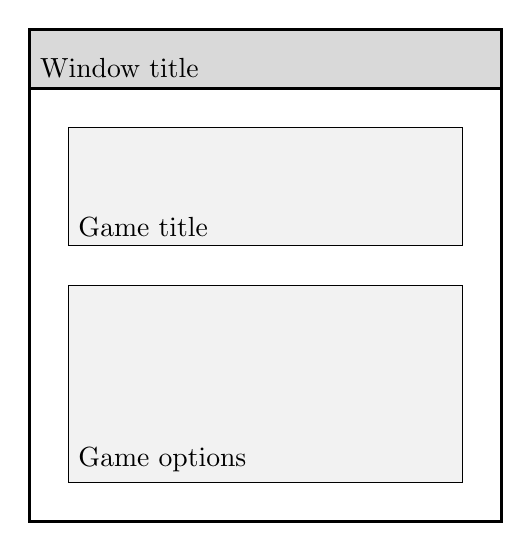
\begin{tikzpicture}
	\draw[very thick,fill=black!15] (0,5.5) node[anchor=south west]{Window title} rectangle +(6,.75);
	\draw[very thick] (0,0)  rectangle +(6,5.5);
	\draw[fill=black!5] (.5,3.5) node[anchor=south west]{Game title} rectangle +(5,1.5);
	\draw[fill=black!5] (.5,.5) node[anchor=south west]{Game options} rectangle +(5,2.5);
	\end{tikzpicture}\hspace{.5cm}
	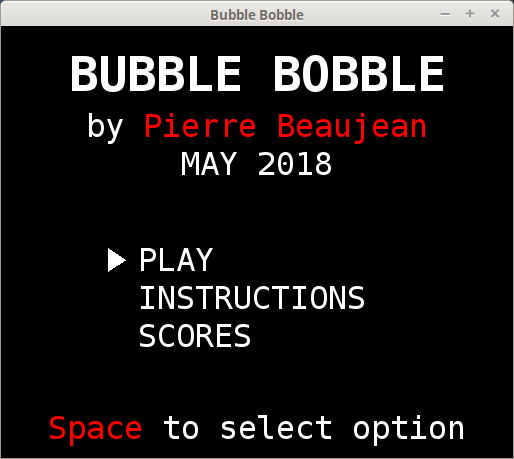
\includegraphics[width=.45\linewidth]{i/screen1}
	
	\caption{Welcome screen of the game (sketch on the left, actual implementation on the right).}
	\label{fig:1:welcome}
\end{figure}

The control screen is given in Figure \ref{fig:2:controls}: there is a title to indicate what the player sees, and some text.

\begin{figure}[!h]
	\centering
	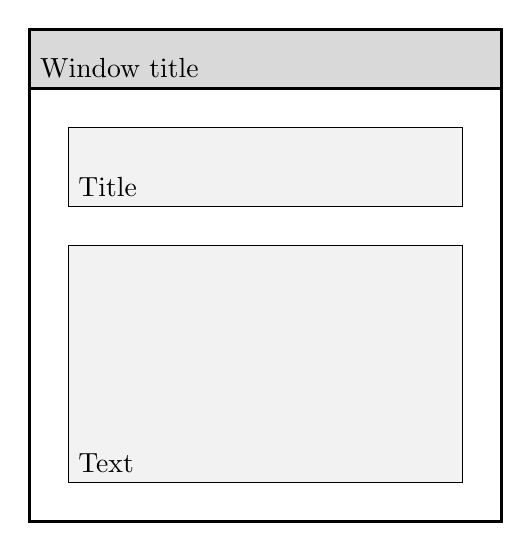
\begin{tikzpicture}
	\draw[very thick,fill=black!15] (0,5.5) node[anchor=south west]{Window title} rectangle +(6,.75);
	\draw[very thick] (0,0)  rectangle +(6,5.5);
	\draw[fill=black!5] (.5,4) node[anchor=south west]{Title} rectangle +(5,1);
	\draw[fill=black!5] (.5,.5) node[anchor=south west]{Text} rectangle +(5,3);
	\end{tikzpicture}\hspace{.5cm}
		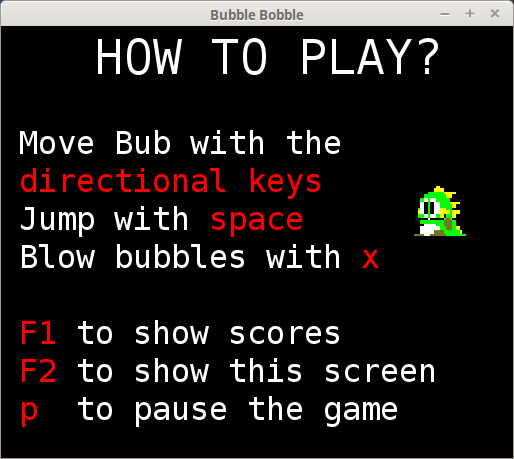
\includegraphics[width=.45\linewidth]{i/screen2}
	\caption{Controls and score screen of the game (sketch on the left, actual implementation on the right).}
	\label{fig:2:controls}
\end{figure}

The score screen is given in Figure \ref{fig:3:score}. In this screen, the score are continuously going up, and the list is repeated. 

\begin{figure}[!h]
	\centering
	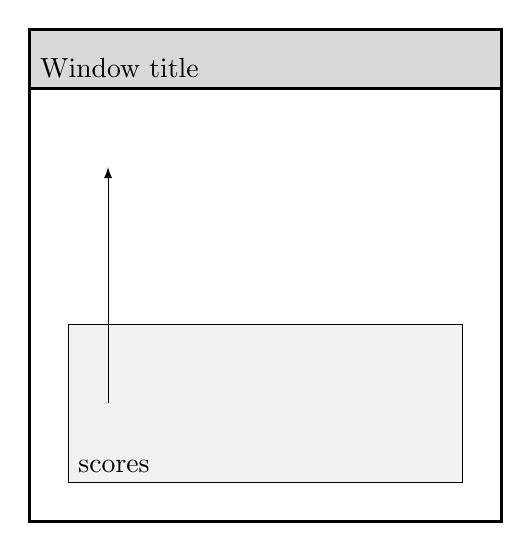
\begin{tikzpicture}
	\draw[very thick,fill=black!15] (0,5.5) node[anchor=south west]{Window title} rectangle +(6,.75);
	\draw[very thick] (0,0)  rectangle +(6,5.5);
	\draw[fill=black!5] (.5,.5) node[anchor=south west]{scores} rectangle +(5,2);
	\draw [-latex] (1,1.5) -- +(0, 3);
	\end{tikzpicture}\hspace{.5cm}
		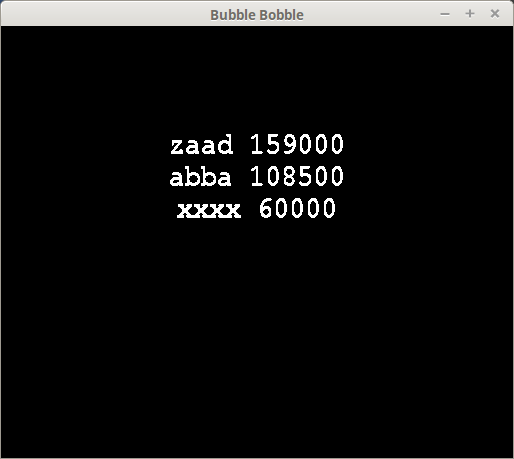
\includegraphics[width=.45\linewidth]{i/screen3}
	\caption{Score screen of the game (sketch on the left, actual implementation on the right).}
	\label{fig:3:score}
\end{figure}

The game over/final screen is given in Figure \ref{fig:3:gameover}. This screen gives the possibility to enter a name associated with the score. If it is game over, the possibility to save the score is not given.

\begin{figure}[!h]
	\centering
	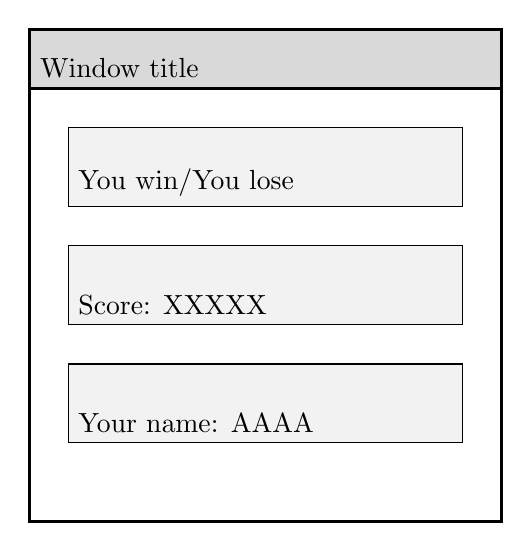
\begin{tikzpicture}
	\draw[very thick,fill=black!15] (0,5.5) node[anchor=south west]{Window title} rectangle +(6,.75);
	\draw[very thick] (0,0)  rectangle +(6,5.5);
	\draw[fill=black!5] (.5,4) node[anchor=south west]{You win/You lose} rectangle +(5,1);
	\draw[fill=black!5] (.5,2.5) node[anchor=south west]{Score: XXXXX} rectangle +(5,1);
	\draw[fill=black!5] (.5,1) node[anchor=south west]{Your name: AAAA} rectangle +(5,1);
	%\draw[fill=black!5] (.5,.5) node[anchor=south west]{Text} rectangle +(5,3);
	\end{tikzpicture} \\
	\vspace{.5cm}
			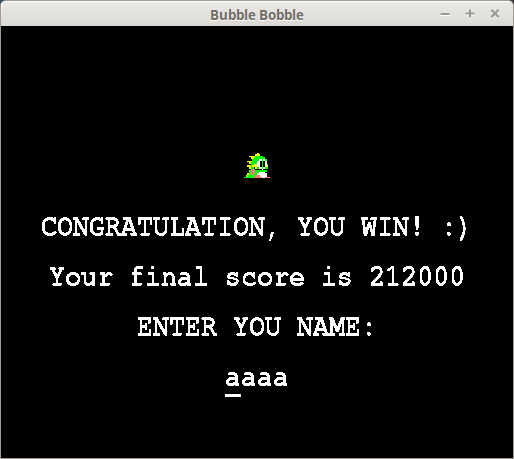
\includegraphics[width=.45\linewidth]{i/screen4}\hspace{.5cm}
			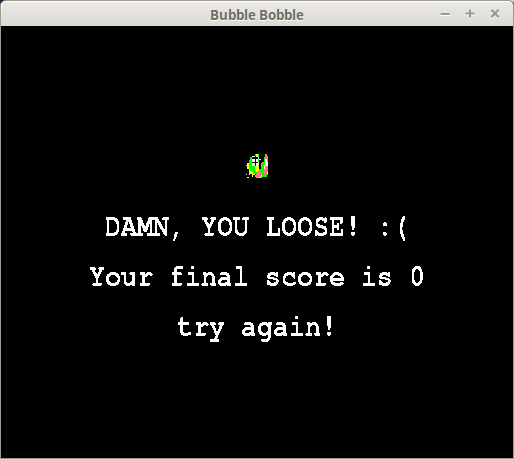
\includegraphics[width=.45\linewidth]{i/screen4b}
	\caption{Game over/final screen of the game (sketch on top, actual implementation on bottom). The player can associate a (four letters) name to its score.}
	\label{fig:3:gameover}
\end{figure}

Finally, the game screen is given in Figure \ref{fig:4:game}. This screen is subdivided in 32$\times$27 squares of 16$\times$16 px (the two top rows being outside of the actual gaming area). Each square is either \textbf{empty} (black) or \textbf{filled} (with a tile image), to represent a physical wall/platform. An actual map is actually 32$\times$24, since the last line is exactly the same as the first one (so that if a dragon/monster fall in the bottom, it can reappear in the top). An map object (item, dragon, monster) is a $2\times2$ square.

%A dragon or a monster move by one square at the time on the left and the right, if there is no filled square in the way. Its jump is of 6 squares up. When it jumps, the dragon/monster  goes up first (whether or not there is filled squares in the way), then go down and stops in an empty square, if there is a filled square below (otherwise, it continues to fall). The position of Bub is always the same at the beginning of the level and when they lose a life (see Figure \ref{fig:4:game}). The position of the monster depends on the level (at the beginning of the level, they fall from the top to a given position in the level, then starts to move).

% The movement of a bubble is very specific: it starts by going in the direction it has been blown, until it loses its \textit{momentum}. When it does, all the bubbles end up in about the same position in the level, by going up/down first, then left/right. Bubbles burst on their own after a time, freeing the monster that they contain if it was the case.

\begin{figure}[!h]
	\centering
	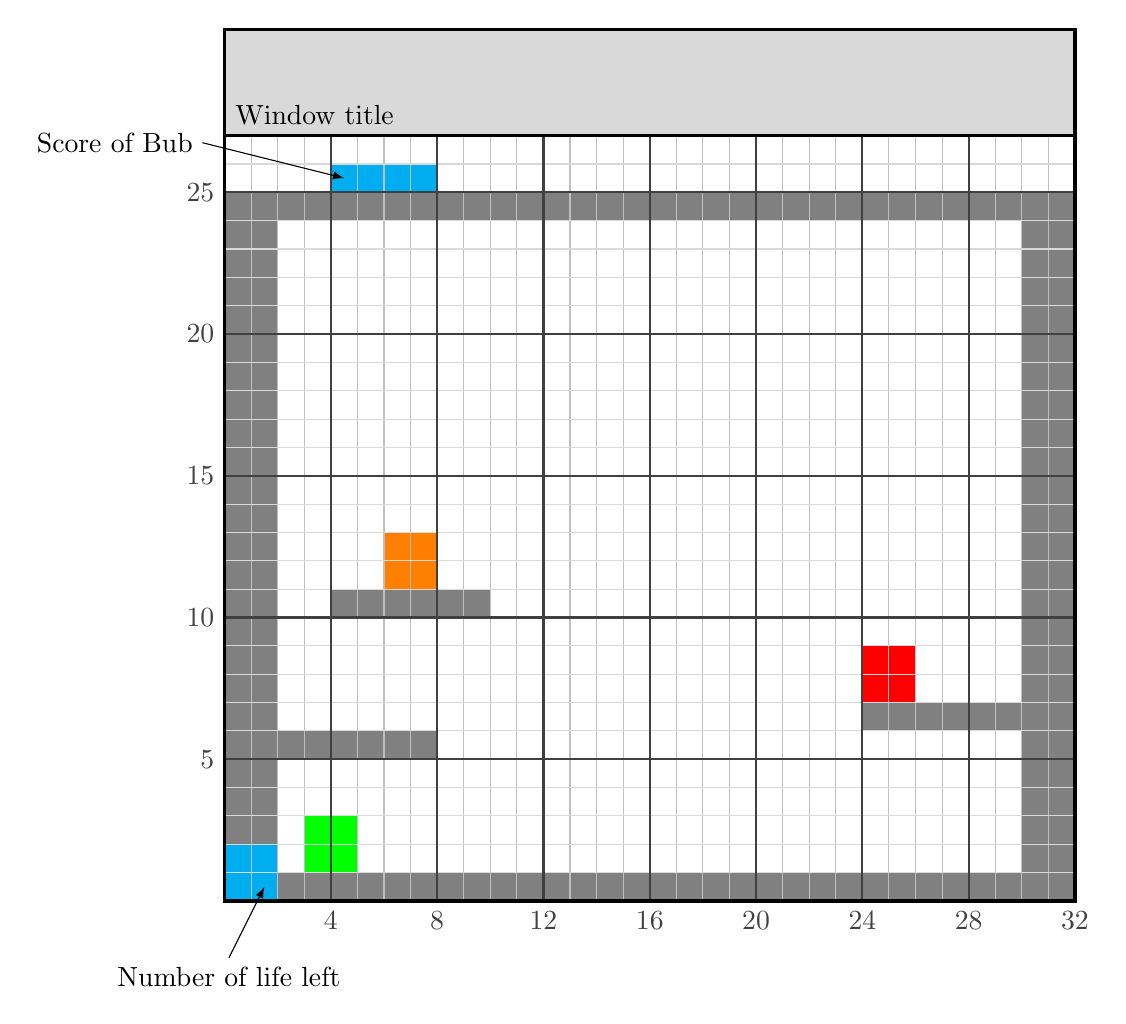
\begin{tikzpicture}[scale=.9]
	% wall
	\fill[black!50] (0,0) rectangle +(.75,10);
	\fill[black!50] (11.25,0) rectangle +(.75,10);
	\fill[black!50] (.75,0) rectangle +(11.25,.4);
	\fill[black!50] (.75,9.6) rectangle +(11.25,.4);
	
	% platform
	\fill[black!50] (.75,2) rectangle +(2.25,.4);
	\fill[black!50] (1.5,4) rectangle +(2.25,.4);
	
	\fill[black!50] (9,2.4) rectangle +(2.25,.4);
	
	% bub&bob
	\filldraw[green] (1.125,.4) rectangle +(.75,.8);
	%\filldraw[blue] (10.125,.4) rectangle +(.75,.8);
	
	% monster & item
	\filldraw[orange] (2.25,4.4) rectangle +(.75,.8);
	\filldraw[red] (9.,2.8) rectangle +(.75,.8);
	
	% info
	\filldraw[cyan] (0,0) rectangle +(.75,.8);
	%\filldraw[cyan] (11.25,0) rectangle +(.375,.4);
	
	\filldraw[cyan] (1.5,10) rectangle +(1.5,.4);
	
	%\filldraw[cyan] (9,10) rectangle +(1.5,.4);
	
	%\filldraw[cyan] (5.625,9.6) rectangle +(.75,.4);
	
	% grid
	\foreach \i in {1,2,...,31}{
		\draw[black!25] (\i*.375,0) -- +(0,11);
	}  
	\foreach \i in {1,2,...,26}{
	\draw[black!15] (0,.4*\i) -- +(12,0);
	} 

	\foreach \i in {4,8,...,32}{
	\draw[black!75,thick] (\i*.375,0) node[below]{\i} -- +(0,11);
	}  
	\foreach \i in {5,10,...,25}{
		\draw[black!75,thick] (0,.4*\i) node[left]{\i} -- +(12,0);
	} 

	\draw[very thick,fill=black!15] (0,10.8) node[anchor=south west]{Window title} rectangle +(12,1.5);
	\draw[very thick] (0,0)  rectangle +(12,10.8);
	
	\draw[latex-] (.375+.5*.375,0+.2) -- +(-.5,-1) node[below]{Number of life left};
	%\draw[latex-] (11.25+.5*.375,0+.2) -- +(.5,-1) node[below]{Number of life left (Bob)};
	\draw[latex-] (1.5+.5*.375,10+.2) -- +(-2,.5) node[left]{Score of Bub};
	%\draw[latex-] (10.125+.5*.375,10+.2) -- +(2,.5) node[right]{Score of Bob};
	%\draw[latex-] (5.625+.5*.375,9.6+.2) -- +(0,3) node[above]{Level number};
	
	\end{tikzpicture}
	
	\vspace{.5cm}
	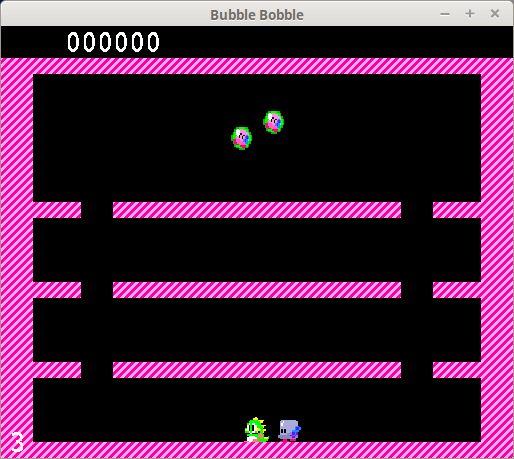
\includegraphics[width=.5\linewidth]{i/screen5}
	
	\caption{Game screen (sketch on top, actual implementation on bottom) subdivided in 32$\times$27 squares. Filled square represent wall/platform. The starting position of Bub is represented by the green square. The orange square represents an item, which Bub is able to grab by jumping on the first, then the second platform (since they are spaced by 5 squares), while Bob will not be able to reach the platform on top of him (since it is 6 squares up). On the other hand, the monster (red square) is able to jump down and try to touch Bob. The position of some extra information (score, life left) are given in lighter blue.}
	\label{fig:4:game}
\end{figure}


\subsection{Modules: data structures and main functions}

\subsubsection{Preamble: conventions}

\begin{figure}[!p]
\centering
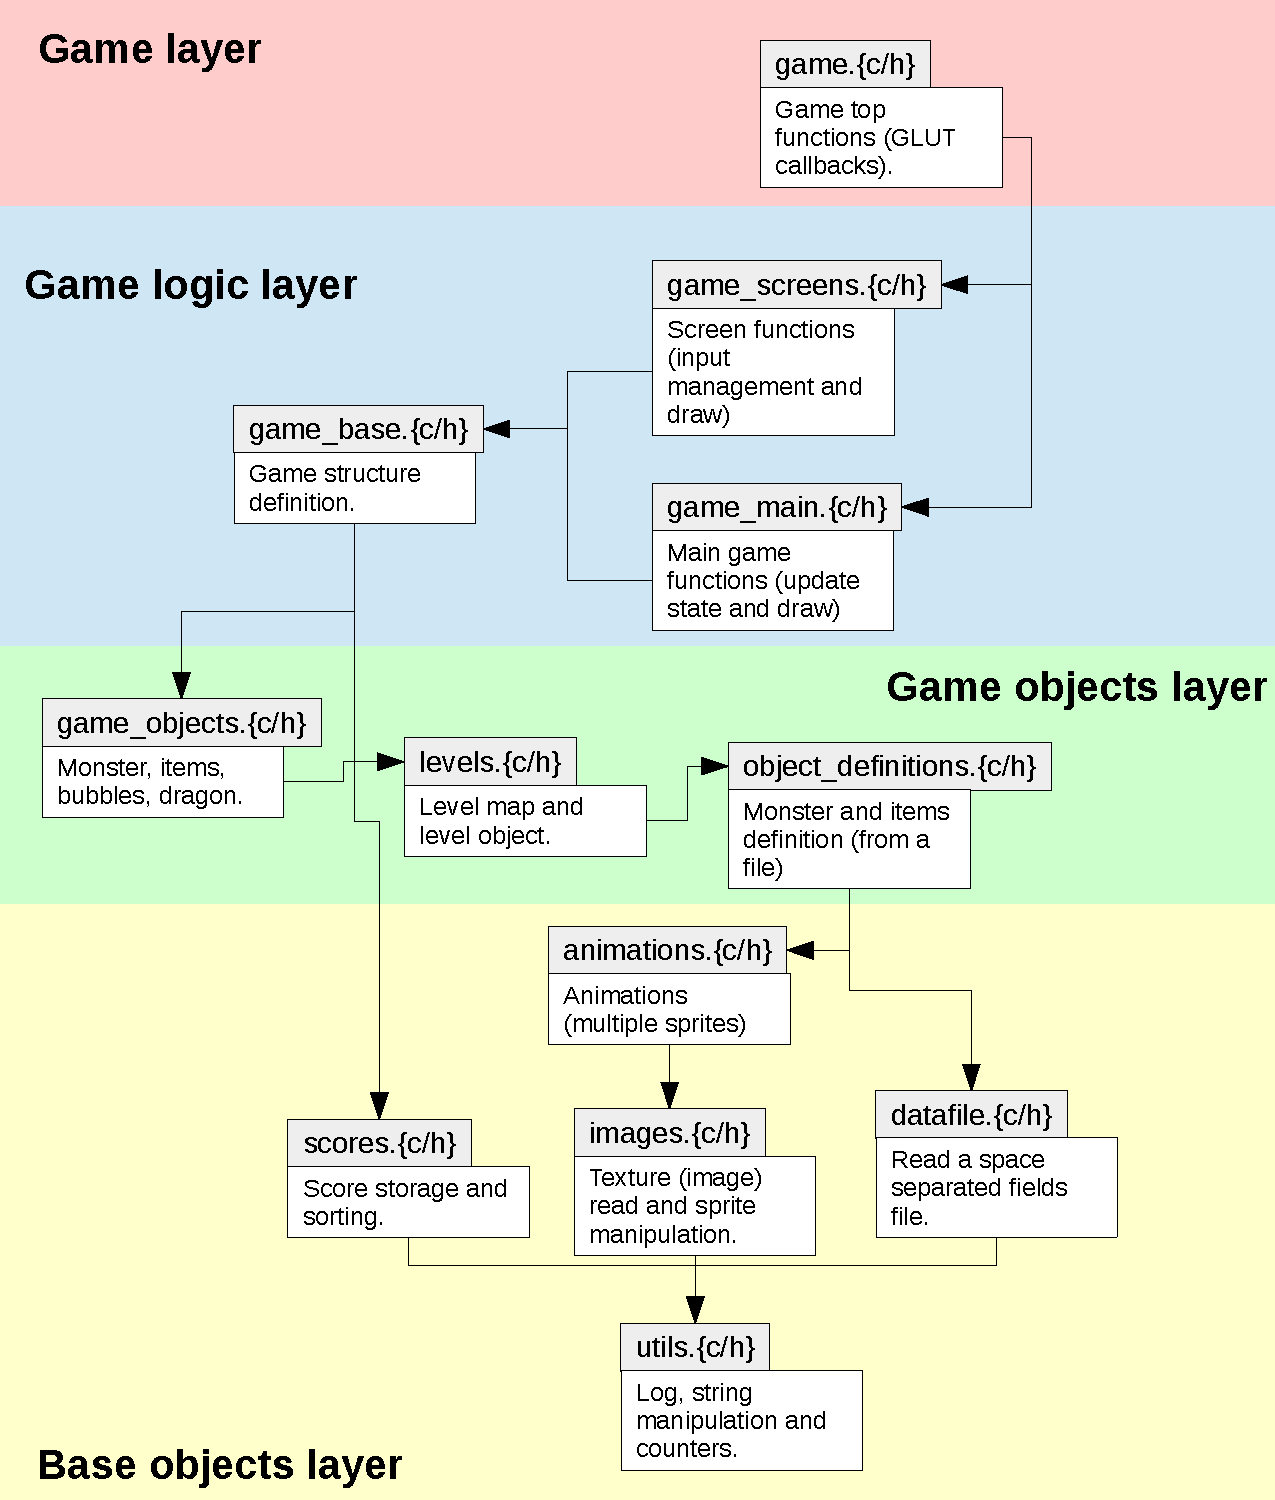
\includegraphics[width=.8\linewidth]{i/files}
\caption{Module organisation and main features of those modules. The arrows show what is included in each module.}
\label{fig:modules}
\end{figure}

The following parts will follow these conventions:

\begin{itemize}
\item The module (divided into 4 layers) are organized as presented in Figure \ref{fig:modules}. The bottom layer contains all the methods and structure for basic manipulation (of images, files and score). Then, the game object layer contains methods and structures that make sense in the game (the map, the monsters, the bubbles, the items and the dragon). The following layer (game logic) gathers all the objects together and deals with how they interact together, as well as their responses to inputs (only for the dragon or the screens). Finally the last layer (game) contains the interactions with GLUT (with all the callbacks that it needs). The following pages will present the different modules from the bottom to the top.
\item The \mintinline{c}{*_new()}  (and \mintinline{c}{*_new_from_file()}) type functions will perform the necessary \mintinline{c}{malloc()} and initialize the structure(s), while the \mintinline{c}{*_delete()} type functions will perform the required \mintinline{c}{free()}'s.
\item The program will log a certain number of informations in order to be able to detect and fix a crash.
\item A chained list corresponds to the following representation:\begin{center}
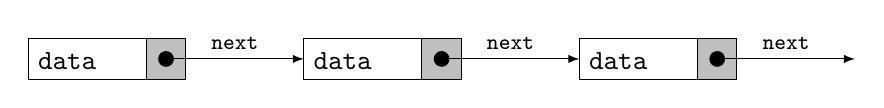
\begin{tikzpicture}
\foreach\i in {0,1,2} {
\begin{scope}[xshift=\i*3.5cm]
\draw (0,0) node[anchor=south west]{\texttt{data}} rectangle +(1.5,1.5em);
\draw[fill=black!25] (1.5,0) rectangle +(.5,1.5em);
\fill (1.75,.75em) circle (.1cm);
\draw[-latex] (1.75,.75em) -- node[above]{\footnotesize\texttt{next}} +(1.75,0);
\end{scope}
}
\end{tikzpicture}
\end{center}
where \mintinline{c}{data} is a block of data and \text{next} a pointer to the next element of the list. It is a \mintinline{c}{NULL} terminated chained list if the last element is set to \mintinline{c}{NULL}, while it is circular if the last element point to the first element of the chain. Notice that in the case of circular lists, a sentinel is needed: \begin{center}
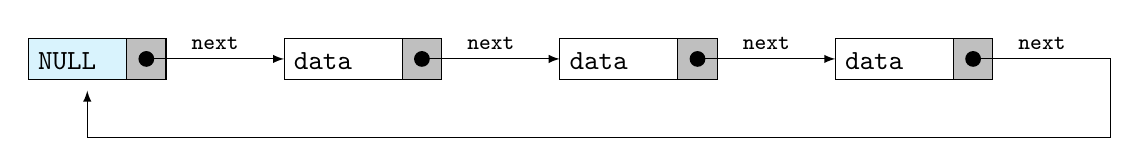
\begin{tikzpicture}
\draw[fill=cyan!15]  (-3.25,0) node[anchor=south west]{\texttt{NULL}} rectangle +(1.5,1.5em);
\draw[fill=black!25] (-2,0) rectangle +(.5,1.5em);

\foreach\i in {0,1,2} {
\begin{scope}[xshift=\i*3.5cm]
\draw (0,0) node[anchor=south west]{\texttt{data}} rectangle +(1.5,1.5em);
\draw[fill=black!25] (1.5,0) rectangle +(.5,1.5em);
\fill (-1.75,.75em) circle (.1cm);
\draw[latex-] (0,.75em) -- node[above]{\footnotesize\texttt{next}} +(-1.75,0);
\end{scope}
}
\fill (8.75,.75em) circle (.1cm);
\draw[-latex] (8.75,.75em) -- node[above]{\footnotesize\texttt{next}} ++(1.75,0) -- ++(0,-1) -- ++(-13, 0) -- ++(0,1.7em);
\end{tikzpicture}
\end{center}
The sentinel (blue in the scheme above) is always the first element of the list, and the data is set to \mintinline{c}{NULL}.
\item All files used here (except image files) will be text files. Each of these files will contain multiple lines with values in it. Each value is space-separated. To define a file format, the following representation will be used:\begin{center}
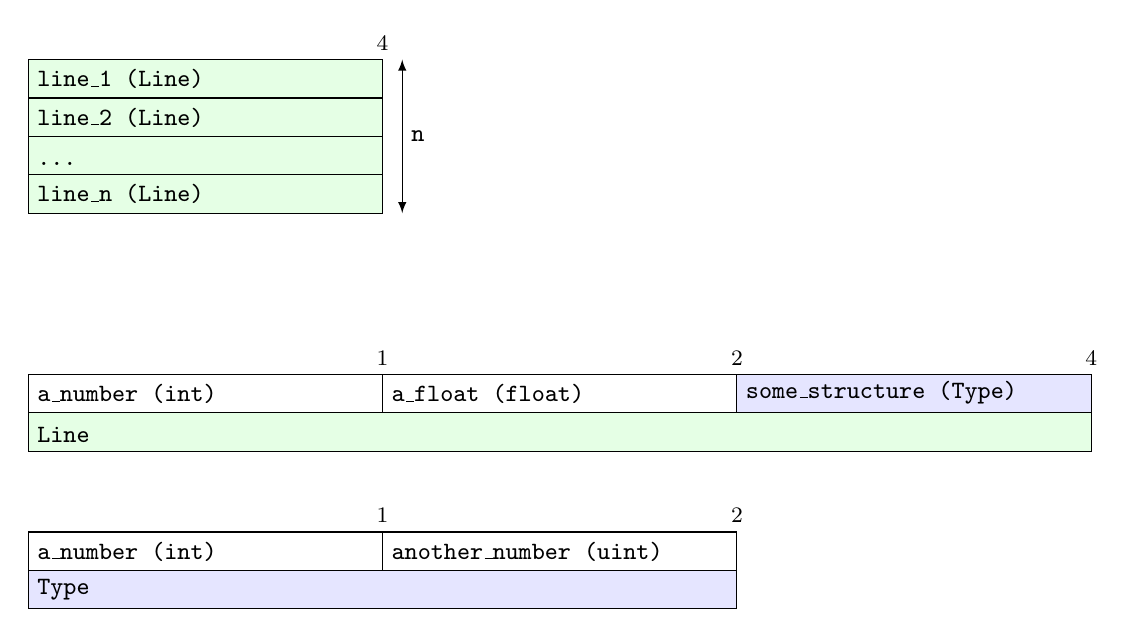
\begin{tikzpicture}
\small
\def\sz{4.5}

\draw[fill=green!10] (0,4) node[anchor=south west]{\texttt{line\_1 (Line)}} rectangle +(\sz,1.5em) node[above]{\footnotesize 4};
\draw[fill=green!10] (0,4cm-1.5em) node[anchor=south west]{\texttt{line\_2 (Line)}} rectangle +(\sz,1.5em);
\draw[fill=green!10] (0,4cm-3em) node[anchor=south west]{\texttt{...}} rectangle +(\sz,1.5em);
\draw[fill=green!10] (0,4cm-4.5em) node[anchor=south west]{\texttt{line\_n (Line)}} rectangle +(\sz,1.5em);

\draw[latex-latex] (\sz cm+.25cm,4cm+1.5em) -- node[right]{\texttt{n}} +(0,-6em);


\draw (0,0) node[anchor=south west]{\texttt{a\_number (int)}} rectangle +(\sz,1.5em) node[above]{\footnotesize 1};
\draw (1*\sz,0) node[anchor=south west]{\texttt{a\_float (float)}} rectangle +(\sz,1.5em) node[above]{\footnotesize 2};
\draw[fill=blue!10]  (2*\sz,0) node[anchor=south west]{\texttt{some\_structure (Type)}} rectangle +(\sz,1.5em) node[above]{\footnotesize 4};
\draw[fill=green!10] (0,-1.5em) node[anchor=south west]{\texttt{Line}} rectangle +(3*\sz,1.5em);

\draw (0,-2) node[anchor=south west]{\texttt{a\_number (int)}} rectangle +(\sz,1.5em) node[above]{\footnotesize 1};
\draw (\sz,-2) node[anchor=south west]{\texttt{another\_number (uint)}} rectangle +(\sz,1.5em) node[above]{\footnotesize 2};
\draw[fill=blue!10] (0,-2cm-1.5em) node[anchor=south west]{\texttt{Type}} rectangle +(2*\sz,1.5em);
\end{tikzpicture}
\end{center}
Each block represents information. Vertically aligned blocks are on the same line. If a block contains more than one value (which correspond generally to a structure), the block is colored, and its definition is given below (here for \texttt{Line}, in green, and \texttt{Type}, in blue). Ultimately, that represent values, separated to the next by a space (for example, each line of the file is actually represented by 4 values in this example). Above the end of each block, there is a counter of the number of values so far in the line.
Here, the first blocks represent the file, with \texttt{n} lines (indicated by the arrow on the right). Note that \texttt{uint} will be used as the shorthand for \mintinline{c}{unsigned int}.
\item I will assume  a fixed framerate of 60 frames per second (since it is the vertical synchronization value of most of the modern screens). Every time length will therefore be expressed in a number of frames. 
\item The code does not contains any unit test. This is clearly bad, but as much as I like unit testing\footnote{I usually program in Python, where this kind of thing is easier to implement and manage}, it is clearly difficult to do in C\footnote{Of course there is dedicated framework to do so (Google test, for example), but it goes beyond the scope of this project, I think.}, especially with graphical interfaces.
\end{itemize}

\subsubsection{Misc (\texttt{utils.h})}

\subsubsection{Images (\texttt{textures.h})}

Since the game will need to manipulate images, it may be interesting to define three kinds of structures that represent \begin{inparaenum}[i)]
\item a pixel (with a red, green and blue value and a transparency to know whether the pixel should be drawn or not), 
\item a texture (a array of pixels), and
\item a sprite (a part of a texture, for example the image of an object).
\end{inparaenum}

\begin{minted}[breaklines]{c}
typedef struct Pixel_ {
	// each color value is between 0 (black) and 255 (full color)
	unsigned char red;
	unsigned char green;
	unsigned char blue;
	bool transparent; // "true" if the pixel is transparent 
} Pixel;

typedef struct Texture_ {
	unsigned int width;
	unsigned int height;
	Pixel* pixels; // dynamically allocated
} Texture;

Texture* texture_new_from_file(FILE* f);
void texture_delete(Texture* texture);

Texture* texture_new_from_text(char* text, Texture* sprite_font);

typedef struct Sprite_ {
	Texture* texture; // pointer to the texture
	unsigned int x;
	unsigned int y;
	unsigned int width;
	unsigned int height;
} Sprite;

Sprite* sprite_new(Texture* texture, unsigned int x, unsigned int y, unsigned int w, unsigned int h);
void sprite_delete(Sprite* sprite);
\end{minted}

The strategy is to have a few textures that contains all the sprites needed: for example, a texture for the items, one for the monsters, one for the level tiles, etc. Then, only the sprites are manipulated by the program.

The creation of a texture from a file (using \mintinline{c}{texture_new_from_file()}) is a complex problem, due to the diversity of image formats. To avoid the use of an external library, I will use either PCX \cite{pcx_spec} or BMP \cite{bmp_spec} format, which are two relatively simple image formats to implement (the choice will actually depend on whether it is difficult to export them with GIMP and which is the specification it is actually following).

The \mintinline{c}{texture_new_from_text()} function create a new image containing a text defined as parameters, using a \textit{sprite font}, i.e. an image where the letters are located in a known position (see, for example, Figure \ref{fig:def:spritefont}). The image will be created by copying the pixels corresponding to each letter. \footnote{Even though GLUT seems to possess a function to draw a character \cite{glutrefchar}, so I will see whether I use this method or the one that I propose.}

\begin{figure}[!h]
\centering
\includegraphics[width=.5\linewidth]{font-map-sprite}
\caption{Examples of sprite font, with the grid used to locate the different letters \cite{dafont}.}
\label{fig:def:spritefont}
\end{figure}

Note that, since I'm not a good graphic artist (and this is not the goal of the work, anyway), I will use sprites available on the internet, for example from Spriters-Ressource \cite{spriters}.

\subsubsection{Scores (\texttt{scores.h})}

The game needs to store and load scores.

\begin{minted}{c}
typedef struct Score_ {
	char name[4];
	unsigned int score;
	Score* next;
} Score;

Score* score_new(char name[4], unsigned int score);
void score_delete(Score* score);

Score* scores_from_file(FILE* f);
void scores_insert(char name[4], unsigned int score);
Score* scores_store_in_file(FILE* f, Score* list);
void scores_delete(Score* list);
\end{minted}

Following the traditional arcade games, the name will be written with four (uppercase) letters. This is a chained list, loaded from a file (with the \mintinline{c}{scores_from_file()} function) for which the definition is given in Figure \ref{fig:def:scores}. Note that this function order the scores by decreasing value, and insertion (\mintinline{c}{scores_insert()}) will be done in the correct position in this ordered list. The \mintinline{c}{scores_store_in_file()} function is used to store the scores list in the file.

\begin{figure}[!p]
	\centering
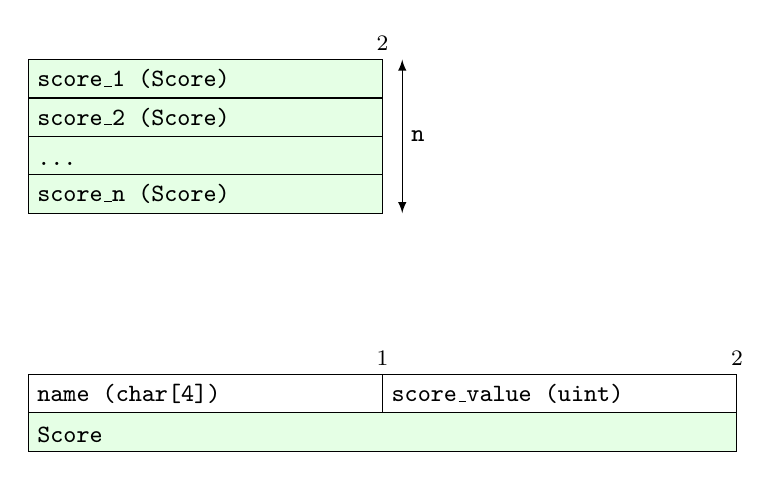
\begin{tikzpicture}
\small
\def\sz{4.5}

\draw[fill=green!10] (0,4) node[anchor=south west]{\texttt{score\_1 (Score)}} rectangle +(\sz,1.5em) node[above]{\footnotesize 2};
\draw[fill=green!10] (0,4cm-1.5em) node[anchor=south west]{\texttt{score\_2 (Score)}} rectangle +(\sz,1.5em);
\draw[fill=green!10] (0,4cm-3em) node[anchor=south west]{\texttt{...}} rectangle +(\sz,1.5em);
\draw[fill=green!10] (0,4cm-4.5em) node[anchor=south west]{\texttt{score\_n (Score)}} rectangle +(\sz,1.5em);

\draw[latex-latex] (\sz cm+.25cm,4cm+1.5em) -- node[right]{\texttt{n}} +(0,-6em);


\draw (0,0) node[anchor=south west]{\texttt{name (char[4])}} rectangle +(\sz,1.5em) node[above]{\footnotesize 1};
\draw (1*\sz,0) node[anchor=south west]{\texttt{score\_value (uint)}} rectangle +(\sz,1.5em) node[above]{\footnotesize 2};
\draw[fill=green!10] (0,-1.5em) node[anchor=south west]{\texttt{Score}} rectangle +(2*\sz,1.5em);
\end{tikzpicture}
\caption{Definition of the file to store scores.}
\label{fig:def:scores}
\end{figure} 

\subsubsection{Definitions of game object types (\texttt{game\_object\_definitions.h})}

Used to define and list the properties of a given type of item or monster. The game engine will use a pointer to refer to those definitions when creating and using an actual item or monster.

\begin{minted}[breaklines]{c}
// items
typedef enum extra_power_t_ {
	EP_NONE,
	EP_ADD_LIFE,
	EP_ADD_EXTRA_LIFE,
	// some other powers
	EP_NUMBER
} extra_power_t;

typedef struct ItemDef_ {
	unsigned int points_given;
	Sprite* sprite;
	extra_power_t extra_power;
} ItemDef;


ItemDef* item_def_new(unsigned int points_given, Sprite* sprite, extra_power_t extra_power);
void item_def_delete(ItemDef* item);

ItemDef** item_defs_from_file(FILE* f, Texture* items_texture, unsigned int* size);

// monsters
typedef struct MonsterDef_ {
	Sprite* sprite_animation[2];  // two sprites for the animation
	unsigned int speed; // number of frames between two movements
} MonsterDef;

MonsterDef* monster_def_new(Sprite* sprite_animation[2], unsigned int speed);
void imonster_def_delete(MonsterDef* item);

MonsterDef** monster_defs_from_file(FILE* f, Texture* items_texture, unsigned int* size);
\end{minted}


The last functions for each structure (\mintinline{c}{*_defs_from_file()}) loads and return an array of item (monster) definitions (of \mintinline{c}{size} elements) defined in a text file. There is one item (one monster) per line, defined by the information given in Figure \ref{fig:def:items} (Figure \ref{fig:def:monsters}). The data structure is therefore the one given in Figure \ref{fig:def:tab}, an array of pointers.

\begin{figure}[!p]
	\centering
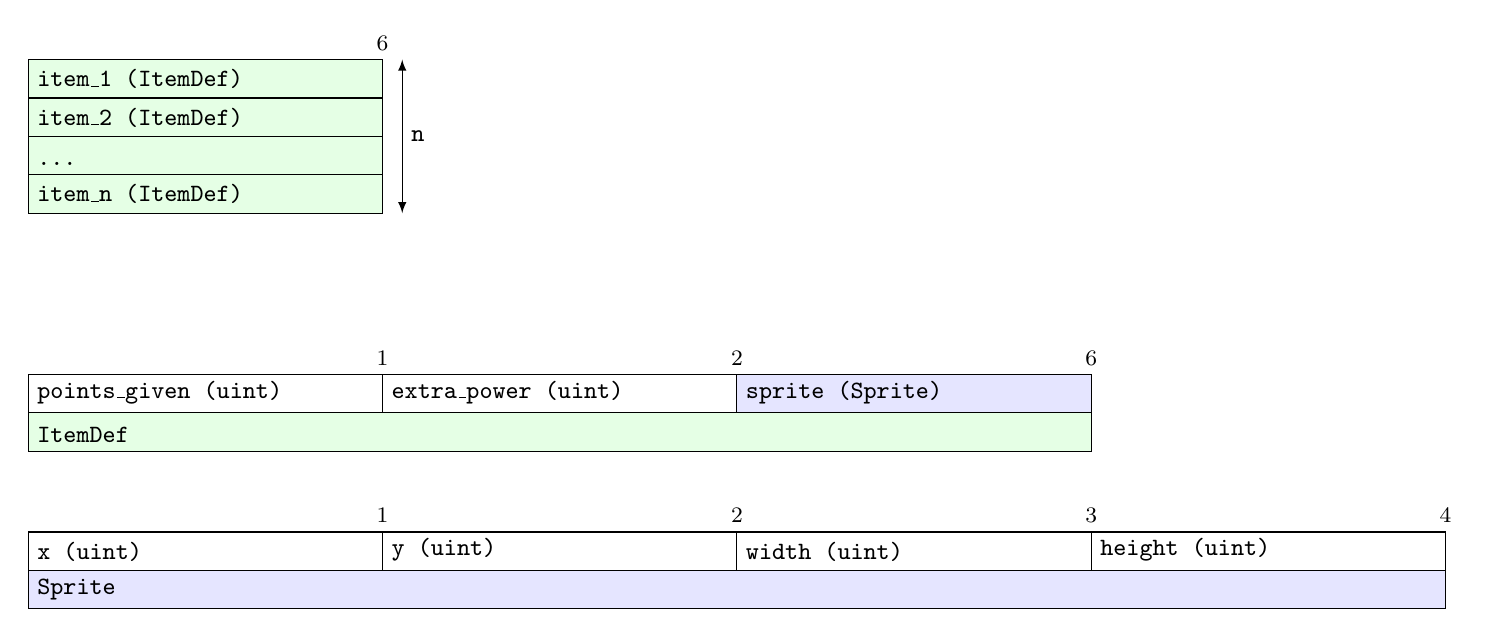
\begin{tikzpicture}
\small
\def\sz{4.5}

\draw[fill=green!10] (0,4) node[anchor=south west]{\texttt{item\_1 (ItemDef)}} rectangle +(\sz,1.5em) node[above]{\footnotesize 6};
\draw[fill=green!10] (0,4cm-1.5em) node[anchor=south west]{\texttt{item\_2 (ItemDef)}} rectangle +(\sz,1.5em);
\draw[fill=green!10] (0,4cm-3em) node[anchor=south west]{\texttt{...}} rectangle +(\sz,1.5em);
\draw[fill=green!10] (0,4cm-4.5em) node[anchor=south west]{\texttt{item\_n (ItemDef)}} rectangle +(\sz,1.5em);

\draw[latex-latex] (\sz cm+.25cm,4cm+1.5em) -- node[right]{\texttt{n}} +(0,-6em);


\draw (0,0) node[anchor=south west]{\texttt{points\_given (uint)}} rectangle +(\sz,1.5em) node[above]{\footnotesize 1};
\draw (1*\sz,0) node[anchor=south west]{\texttt{extra\_power (uint)}} rectangle +(\sz,1.5em) node[above]{\footnotesize 2};
\draw[fill=blue!10]  (2*\sz,0) node[anchor=south west]{\texttt{sprite (Sprite)}} rectangle +(\sz,1.5em) node[above]{\footnotesize 6};
\draw[fill=green!10] (0,-1.5em) node[anchor=south west]{\texttt{ItemDef}} rectangle +(3*\sz,1.5em);

\draw (0,-2) node[anchor=south west]{\texttt{x (uint)}} rectangle +(\sz,1.5em) node[above]{\footnotesize 1};
\draw (\sz,-2) node[anchor=south west]{\texttt{y (uint)}} rectangle +(\sz,1.5em) node[above]{\footnotesize 2};
\draw (2*\sz,-2) node[anchor=south west]{\texttt{width (uint)}} rectangle +(\sz,1.5em) node[above]{\footnotesize 3};
\draw (3*\sz,-2) node[anchor=south west]{\texttt{height (uint)}} rectangle +(\sz,1.5em) node[above]{\footnotesize 4};
\draw[fill=blue!10] (0,-2cm-1.5em) node[anchor=south west]{\texttt{Sprite}} rectangle +(4*\sz,1.5em);
\end{tikzpicture}
\caption{Definition of the file to store item definitions. The \texttt{extra\_power} value will be converted to \texttt{extra\_power\_t}.}
\label{fig:def:items}
\end{figure}

\begin{figure}[!p]
	\centering
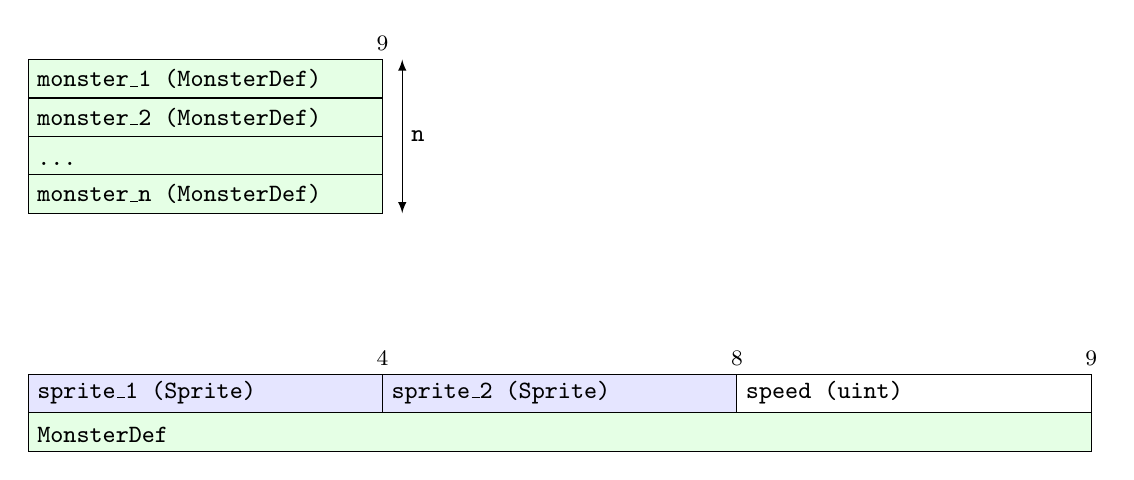
\begin{tikzpicture}
\small
\def\sz{4.5}

\draw[fill=green!10] (0,4) node[anchor=south west]{\texttt{monster\_1 (MonsterDef)}} rectangle +(\sz,1.5em) node[above]{\footnotesize 9};
\draw[fill=green!10] (0,4cm-1.5em) node[anchor=south west]{\texttt{monster\_2 (MonsterDef)}} rectangle +(\sz,1.5em);
\draw[fill=green!10] (0,4cm-3em) node[anchor=south west]{\texttt{...}} rectangle +(\sz,1.5em);
\draw[fill=green!10] (0,4cm-4.5em) node[anchor=south west]{\texttt{monster\_n (MonsterDef)}} rectangle +(\sz,1.5em);

\draw[latex-latex] (\sz cm+.25cm,4cm+1.5em) -- node[right]{\texttt{n}} +(0,-6em);


\draw[fill=blue!10] (0,0) node[anchor=south west]{\texttt{sprite\_1 (Sprite)}} rectangle +(\sz,1.5em) node[above]{\footnotesize 4};
\draw[fill=blue!10]  (1*\sz,0) node[anchor=south west]{\texttt{sprite\_2 (Sprite)}} rectangle +(\sz,1.5em) node[above]{\footnotesize 8};
\draw  (2*\sz,0) node[anchor=south west]{\texttt{speed (uint)}} rectangle +(\sz,1.5em) node[above]{\footnotesize 9};
\draw[fill=green!10] (0,-1.5em) node[anchor=south west]{\texttt{MonsterDef}} rectangle +(3*\sz,1.5em);
\end{tikzpicture}
\caption{Definition of the file to store monster definitions. The \texttt{Sprite} structure (blue) is the same as in Figure \ref{fig:def:items}.}
\label{fig:def:monsters}
\end{figure}

\begin{figure}[!h]
\centering
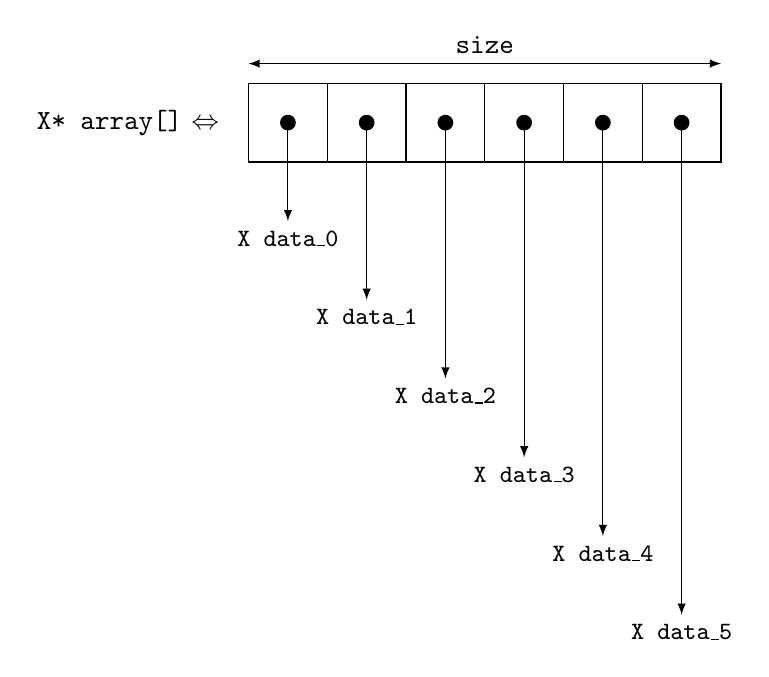
\begin{tikzpicture}
\foreach\i in {0,1,2,3,4,5} {
\draw (\i,0) rectangle +(1,1);
\fill (\i+.5,.5) circle (.1cm);
\draw[-latex] (\i+.5,.5) -- +(0,-1-\i.25) node[below]{\small \texttt{X data\_\i}};
}

\draw (-.25,.5) node[left]{\texttt{X* array[]} $\Leftrightarrow$ };

\draw[latex-latex] (.0,1.25) -- node[midway,above]{\texttt{size}} +(6,0);
\end{tikzpicture}
\caption{Data structure of an array of size \mintinline{c}{size} (here, 5) of pointers to a structure \mintinline{c}{X}.}
\label{fig:def:tab}
\end{figure}

Note that the choice to use arrays here is not innocent, since those definitions will be called via their positions in the table (corresponding to their positions in the file) in the levels (see below).

\subsubsection{Levels (\texttt{levels.h})}

A level contains the map, which could be stored as an array, but it may be more interesting to use a chained list in this case, as pictured in Figure \ref{fig:def:chainx}.

\begin{minted}[breaklines]{c}
enum {
	N_LEFT,
	N_RIGHT,
	N_TOP,
	N_BOTTOM,
	N_NUMBER
};

typedef struct Square_ {
	bool is_filled;
	unsigned short position[2]; // in number of square, i.e. (2,2)
	struct Square_* neighbor[N_NUMBER]; 
} Square;

Square* square_new(bool is_filled, unsigned short position[2], Square* left, Square* right, Square* top, Square* bottom);
void square_delete(Square* square);
\end{minted}

\begin{figure}[!h]
\centering
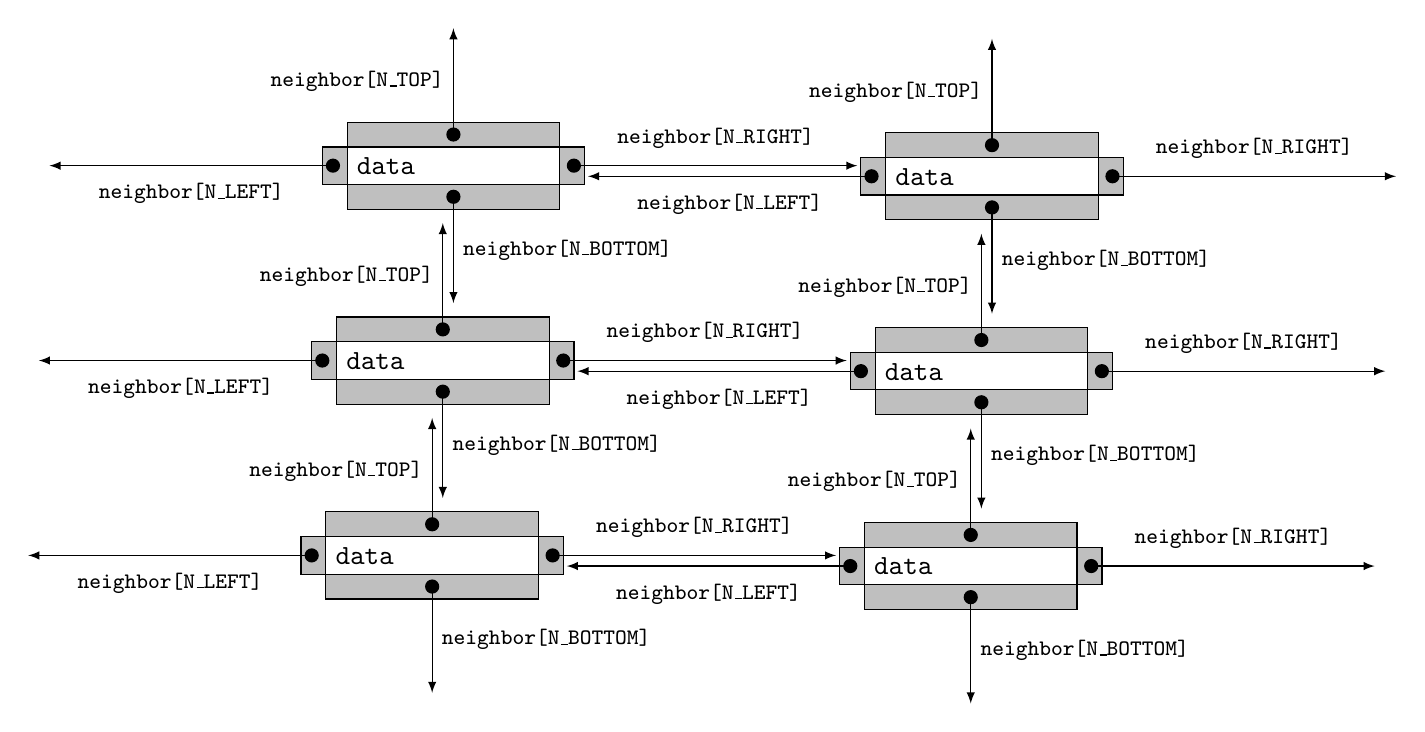
\begin{tikzpicture}[scale=.9]
\foreach\i in {0,1}{
\foreach \j in {0,1,2} {
\begin{scope}[xshift=\i*7.6cm+\j*.15cm,yshift=\j*2.75cm+\i*-.15cm]
\draw (0,0) node[anchor=south west]{\texttt{data}} rectangle +(3,1.5em);
\draw[fill=black!25] (0,1.5em) rectangle +(3,1em);
\fill (1.5,2em) circle (.1cm) ;
\draw[-latex] (1.5,2em) -- node[left]{\footnotesize\texttt{neighbor[N\_TOP]}} +(0,1.5);
\draw[fill=black!25] (0,-1em) rectangle +(3,1em);
\fill (1.5,-.5em) circle (.1cm) ;
\draw[-latex] (1.5,-.5em) -- node[right]{\footnotesize\texttt{neighbor[N\_BOTTOM]}} +(0,-1.5);
\draw[fill=black!25] (3,0) rectangle +(1em,1.5em);
\fill (3.2,.75em) circle (.1cm) ;
\draw[-latex] (3.2,.75em) -- node[above=.1cm]{\footnotesize\texttt{neighbor[N\_RIGHT]}} +(4,0);
\draw[fill=black!25] (0,0) rectangle +(-1em,1.5em);
\fill (-.2,.75em) circle (.1cm) ;
\draw[-latex] (-.2,.75em) -- node[below=.1cm]{\footnotesize\texttt{neighbor[N\_LEFT]}} +(-4,0);
\end{scope}
}
}
\end{tikzpicture}
\caption{Representation of the chained list used for the map: \mintinline{c}{data} is the different data that the structure contains, while the \mintinline{c}{neighbor[]} array contains pointers to the left, right, top and bottom squares.}
\label{fig:def:chainx}
\end{figure}

This quadruple chained list is only circular in its \mintinline{c}{neighbor[N_BOTTOM]} pointer, since the dragons and monsters can end up on the top while going down, but the other chained lists are \mintinline{c}{NULL} terminated. Note that since a \mintinline{c}{Square} represents a case in the map (for which the \mintinline{c}{position} parameter gives the actual position), it can actually be used as a position indicator for the different objects. 

The level also contains the tile used for the filled square, a list of the monster with their initial position, and the final position of the bubble. The \mintinline{c}{Level} structure is, itself, a simple (\mintinline{c}{NULL} terminated) chained list, since it makes sense to go to the next level, but not to the previous one.

\begin{minted}[breaklines]{c}
typedef struct Level_ {
	Square* map; // pointer to the bottom left (0,0) square
	Square* bubble_endpoint;
	Sprite* fill_tile;
	unsigned int num_monsters; 
	MonsterDef* monsters[]; // dynamically allocated
	Square* monster_positions[]; // dynamically allocated
	struct Level_* next; // NULL terminated
} Level;

Level* level_new_from_file(FILE* f);
void level_delete(Level* level);

Level* levels_new_from_file(FILE* f);
void levels_delete(Level* list);
\end{minted}

The \mintinline{c}{level_new_from_file()} function create the level from a \textbf{portion} of a text file, for which the definition is pictured in Figure \ref{fig:def:level}. At the end of this function, the file cursor is set to the next level: since the number of lines is known when the header is read (\text{1 + \mintinline{c}{num_monster} + 24}), it is actually possible to store all levels in a file. The function \mintinline{c}{levels_new_from_file()} read the whole file (by calling \mintinline{c}{level_new_from_file()} repetitively until \mintinline{c}{EOF}) and create the chained list. The \mintinline{c}{levels_delete()} take care of freeing all the elements of the chained list (by calling \mintinline{c}{level_delete()}, which free only a given \mintinline{c}{Level}, and take care of the complex\footnote{By starting at the left bottom corner, all \mintinline{c}{Square} may be deleted by following the \mintinline{c}{neighbor[N_RIGHT]} and then \mintinline{c}{neighbor[N_TOP]} pointers.} task to free all \mintinline{c}{Square} in it).

\begin{sidewaysfigure}
\centering
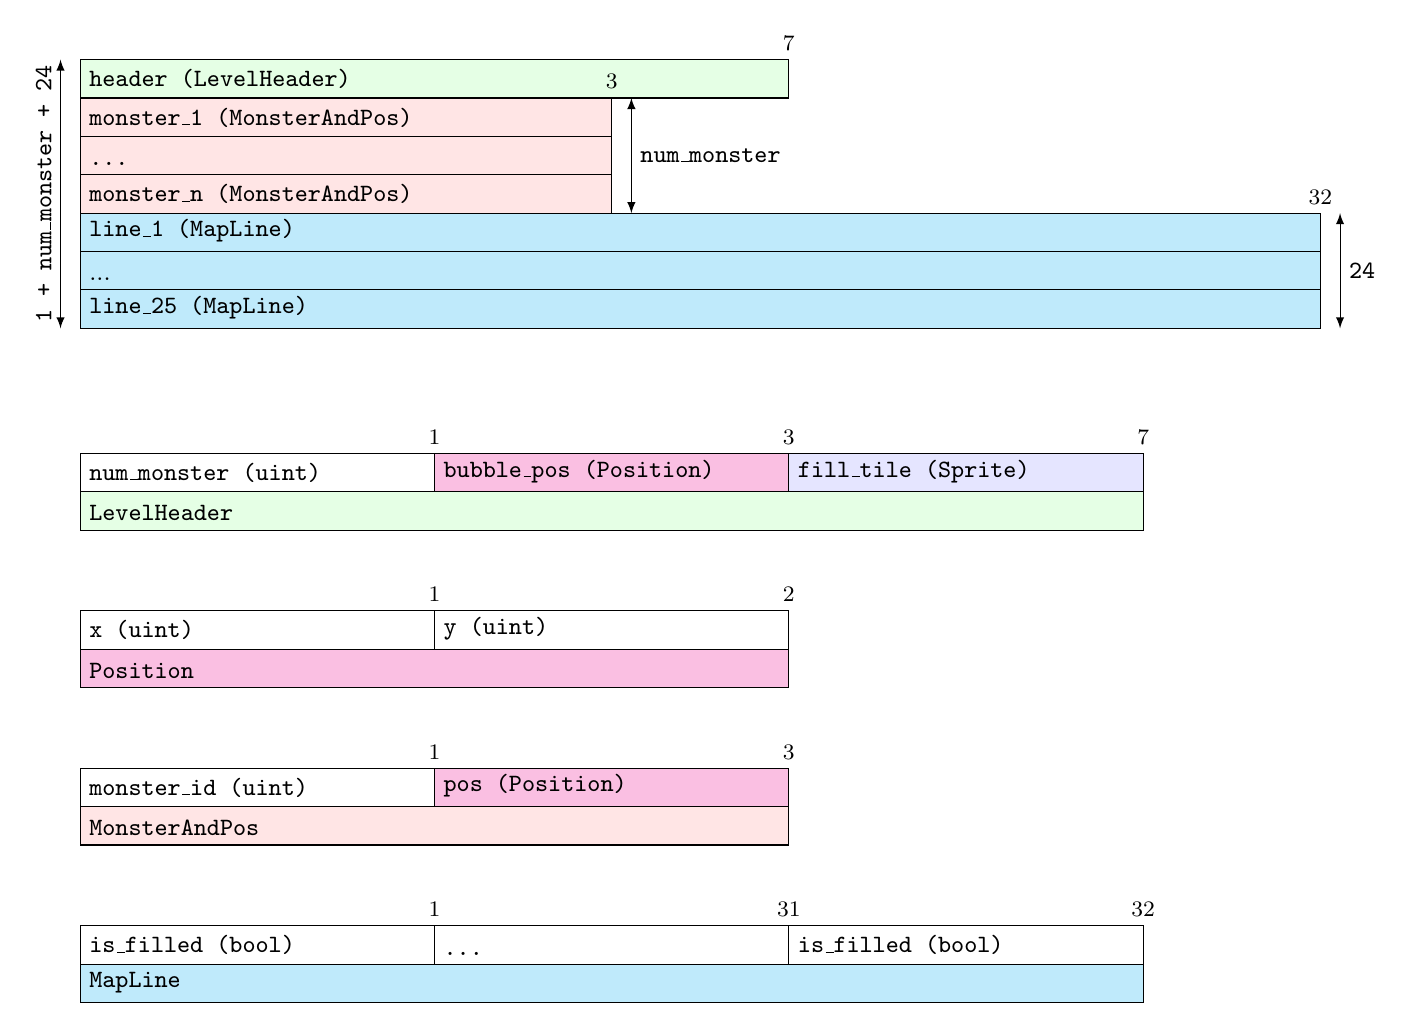
\begin{tikzpicture}
\small
\def\sz{4.5}

\draw[fill=green!10] (0,4) node[anchor=south west]{\texttt{header (LevelHeader)}} rectangle +(2*\sz,1.5em) node[above]{\footnotesize 7};
\draw[fill=red!10] (0,4cm-1.5em) node[anchor=south west]{\texttt{monster\_1 (MonsterAndPos)}} rectangle +(1.5*\sz,1.5em)node[above]{\footnotesize 3};
\draw[fill=red!10] (0,4cm-3em) node[anchor=south west]{\texttt{...}} rectangle +(1.5*\sz,1.5em);
\draw[fill=red!10] (0,4cm-4.5em) node[anchor=south west]{\texttt{monster\_n (MonsterAndPos)}} rectangle +(1.5*\sz,1.5em);
\draw[fill=cyan!25] (0,4cm-6em) node[anchor=south west]{\texttt{line\_1 (MapLine)}} rectangle +(3.5*\sz,1.5em)node[above]{\footnotesize 32};
\draw[fill=cyan!25] (0,4cm-7.5em) node[anchor=south west]{...} rectangle +(3.5*\sz,1.5em);
\draw[fill=cyan!25] (0,4cm-9em) node[anchor=south west]{\texttt{line\_25 (MapLine)}} rectangle +(3.5*\sz,1.5em);

\draw[latex-latex] (1.5*\sz cm+.25cm,4cm) -- node[right]{\texttt{num\_monster}} +(0,-4.5em);
\draw[latex-latex] (3.5*\sz cm+.25cm,4cm-4.5em) -- node[right]{\texttt{24}} +(0,-4.5em);
\draw[latex-latex] (-.25cm,4cm+1.5em) -- node[above,rotate=90]{\texttt{1 + num\_monster + 24}} +(0,-10.5em);


\draw (0,-1) node[anchor=south west]{\texttt{num\_monster (uint)}} rectangle +(\sz,1.5em) node[above]{\footnotesize 1};
\draw[fill=magenta!25] (1*\sz,-1) node[anchor=south west]{\texttt{bubble\_pos (Position)}} rectangle +(\sz,1.5em) node[above]{\footnotesize 3};
\draw[fill=blue!10]  (2*\sz,-1) node[anchor=south west]{\texttt{fill\_tile (Sprite)}} rectangle +(\sz,1.5em) node[above]{\footnotesize 7};
\draw[fill=green!10] (0,-1cm-1.5em) node[anchor=south west]{\texttt{LevelHeader}} rectangle +(3*\sz,1.5em);

\draw (0,-3) node[anchor=south west]{\texttt{x (uint)}} rectangle +(\sz,1.5em) node[above]{\footnotesize 1};
\draw (\sz,-3) node[anchor=south west]{\texttt{y (uint)}} rectangle +(\sz,1.5em) node[above]{\footnotesize 2};
\draw[fill=magenta!25] (0,-3cm-1.5em) node[anchor=south west]{\texttt{Position}} rectangle +(2*\sz,1.5em);

\draw (0,-5) node[anchor=south west]{\texttt{monster\_id (uint)}} rectangle +(\sz,1.5em) node[above]{\footnotesize 1};
\draw[fill=magenta!25] (\sz,-5) node[anchor=south west]{\texttt{pos (Position)}} rectangle +(\sz,1.5em) node[above]{\footnotesize 3};
\draw[fill=red!10] (0,-5cm-1.5em) node[anchor=south west]{\texttt{MonsterAndPos}} rectangle +(2*\sz,1.5em);

\draw (0,-7) node[anchor=south west]{\texttt{is\_filled (bool)}} rectangle +(\sz,1.5em) node[above]{\footnotesize 1};
\draw(\sz,-7) node[anchor=south west]{\texttt{...}} rectangle +(\sz,1.5em) node[above]{\footnotesize 31};
\draw(2*\sz,-7) node[anchor=south west]{\texttt{is\_filled (bool)}} rectangle +(\sz,1.5em) node[above]{\footnotesize 32};
\draw[fill=cyan!25] (0,-7cm-1.5em) node[anchor=south west]{\texttt{MapLine}} rectangle +(3*\sz,1.5em);
\end{tikzpicture}
\caption{Definition of the file to store a level. The \texttt{num\_monster} value (in the \texttt{LevelHeader} structure) is used to determine how many monster lines (\texttt{MonsterAndPos} structures) there will be. The \texttt{monster\_id} value (in \texttt{MonsterAndPos}) refers to the line in the monster definition file. The \texttt{MapLine} structure is repeated 24 times and contains 32 boolean to indicate whether the square is filled or not (since a map is 32$\times$24 squares). The \texttt{Sprite} structure (blue) is the same as in Figure \ref{fig:def:items}.}
\label{fig:def:level}
\end{sidewaysfigure}

\subsubsection{Game objects (\texttt{game\_objects.h})}

Now that the level is defined, the different objects may be as well. Those objects will appear on the screen, on top of the map. The principal attribute that all those objects share is the position. Items and monsters also have a pointer to their definition (to know the sprites, etc.). Finally, they are \mintinline{c}{NULL} terminated chained lists.

\begin{minted}{c}
typedef struct Item_ {
	Square* current_position;
	ItemDef* definition;
	struct Item_* next;
} Item;

Item* item_new(Square* position, ItemDef* definition);
void item_delete(Item* item);

Item* item_new_at_end(Item* list, Square* position, ItemDef* definition);
bool item_delete_in_list(Item* list, Item* element);
void items_delete(Item* list);

typedef struct Monster_ {
	Square* current_position;
	MonsterDef* definition;
	bool invicible; // true at the begining of the game
	bool angry;
	bool in_bubble;
	struct Monster_* next;
} Monster;

Monster* monster_new(Square* position, MonsterDef* definition);
void monster_delete(Monster* monster);

Monster* monster_new_at_end(Monster* list, Square* position, MonsterDef* definition);
bool monster_delete_in_list(Monster* list, Monster* element);
void monsters_delete(Monster* list);

typedef struct Bubble_ {
	Square* current_position;
	unsigned int momentum; // counter until it moves on its own
	unsigned int direction; // N_LEFT or N_RIGHT
	unsigned int time_left; // counter until it auto-burst
	Monster* captured; // NULL in the begining
	struct Bubble_* next; // NULL terminated
} Bubble;

Bubble* bubble_new(Square* position, unsigned int momentum);
void bubble_delete(Bubble* bubble);

Bubble* bubble_new_at_end(Bubble* list, Square* position, unsigned int momentum);
bool bubble_delete_in_list(Bubble* list, Bubble* element);
void bubbles_delete(Bubble* list);
\end{minted}

For those three structures, the  \mintinline{c}{*_new_at_end()} functions add the element at the end of the chained list, while the \mintinline{c}{*_delete_in_list()} functions delete an element in the list (calling \mintinline{c}{*_delete()}) if found (the function returns \mintinline{c}{true} or \mintinline{c}{false} depending if the element is found and deleted or not). Finally, the \mintinline{c}{*s_delete()} functions will delete the whole list.

Concerning the different structure, the \mintinline{c}{Item} one is straightforward. Concerning \mintinline{c}{Monster}, the \mintinline{c}{invincible} parameter is set to \mintinline{c}{true} in the beginning because the monster ``fly" from the top to its initial position. The \mintinline{c}{angry} parameter is a parameter used to determine if the monster is angry: a monster is angry when he was in a bubble and escape because the bubble burst on its own (see below). If this parameter is set to \mintinline{c}{true}, the monster move faster. Finally, the \mintinline{c}{in_bubble} parameter is used to determine if the monster is into a bubble (if so, it is not draw on the screen).

Concerning \mintinline{c}{Bubble}, this structure has a \mintinline{c}{momentum} parameter, which is a counter, decremented at each frame. When this counter is 0, the bubble stops to go in the initial direction (indicated by \mintinline{c}{direction}) and starts to go in the direction of \mintinline{c}{bubble_endpoint} (in \mintinline{c}{Level}, see above). \mintinline{c}{time_left} is another counter, which is decremented at each frame. If this counter is 0, the bubble burst and release the monster (stored in \mintinline{c}{captured}) that it eventually contains (which becomes angry).

A structure to represent the dragons is also needed:

\begin{minted}{c}

// An enum for the dragons animation (DA), 2 frames for each
enum {
	DA_NORMAL_1,
	DA_NORMAL_2,
	DA_BLOW_BUBBLE_1,
	DA_BLOW_BUBBLE_2,
	DA_HIT_1,
	DA_HIT_2,
	BA_DEAD_1,
	BA_DEAD_2,
	DA_INVICIBLE_1,
	DA_INVICIBLE_2
	DA_NUMBER
};

typedef struct Dragon_ {
	Square* current_position;
	unsigned int score;
	unsigned int life; // 3 at the begining
	unsigned int max_life; // 3 at the begining
	bool invicible; // when just killed
	unsigned int invincibility_counter;
	bool is_bub; // if not, this is Bob
	Sprite* animation[DA_NUMBER]; // animations
} Dragon;

Dragon* dragon_new(Square* position, bool is_bub, Sprite* animation[]);
void dragon_delete(Dragon* dragon);
\end{minted}

Indeed, when two players are present, each dragon (player) have its own score and number of life. Also, when a dragon die, if it still have some lives left, it comes back as invincible for a few second (the \mintinline{c}{invicibility_counter} is decremented at each frame, until it gets to 0).

\subsubsection{The game (\texttt{game.h})}

Due to the way that GLUT works \cite{freeglut},  it is required to know whether a keyboard key is pressed or not in the main game loop (see below). To do so, some defines are required :\begin{minted}{c}
#define FRAMES_BETWEEN_KEY_REPEAT 10 // frames

enum {
	E_LEFT,
	E_RIGHT,
	E_TOP,
	E_BOTTOM,
	E_ACTION_1, // i.e. "jump"
	E_ACTION_2, // i.e. "blow"
	E_PAUSE,
	E_SHOW_SCORE,
	E_SHOW_CONTROLS,
	E_QUIT,
	E_SIZE
};
\end{minted}

In the \mintinline{c}{Game} structure (see below), there will be two arrays:\begin{enumerate}
\item A \mintinline{c}{bool key_pressed[E_SIZE]} array. Values are set to \mintinline{c}{true} when a keyboard key is pressed, and \mintinline{c}{false} when released (using \mintinline{c}{glutKeyBoardFunc()} to register the pressed keys and \mintinline{c}{glutKeyboardUpFunc()} to register if they are released \cite{keyb}).
\item A \mintinline{c}{unsigned int key_pressed_interval[E_SIZE]}, which will be set to 0 when a key is pressed, and for which the value will increase at each frame if the key is not up. The goal is to keep track of the amount of time since a key has been pressed, and eventually repeat the event (for example, if the player maintain the direction key pressed) if \mintinline{c}{key_pressed_interval[key] % FRAMES_BETWEEN_KEY_REPEAT == 0}.
\end{enumerate}

The \mintinline{c}{Game} structure will contain everything needed to run the game, and will be instanced once, as one of the (few) global variables.

\begin{minted}{c}
// some defines
#define TIME_INVICIBLE_WHEN_DEAD 50 // 2 secs
#define NUMBER_OF_LIFE 3
#define BUBBLE_TIME 1500 // 25 secs
// (...) I probably forget many of them!

// an enum for the bubbles animations (BA)
enum {
	BA_NORMAL_1,
	BA_NORMAL_2,
	BA_BURST_1,
	BA_BURST_2,
	BA_NUMBER
}

typedef struct Game_ {
	// general stuffs
	bool game_running; // used to pause the game, if any
	bool second_player; // used to know if second player
	bool display_score;
	bool display_controls;
	bool display_welcome;
	// Textures and sprites
	Texture* texture_items;
	Texture* texture_monsters;
	Texture* texture_game;
	Texture* dragon_and_bubbles;
	Texture* texture_sprite_font;
	Sprite* welcome_screen; // for the welcome screen
	Sprite* bubble_animation[BA_NUMBER]; // animations
	// dragons
	Dragon* player_1;
	Dragon* player_2; // may be NULL if no player 2
	// definitions:
	unsigned int num_monster;
	MonsterDef* monster_definitions[];
	unsigned int num_item;
	ItemDef* item_definitions[];
	// levels:
	Level* level_list; // point on the first level
	Level* current_level;
	unsigned int counter_for_next_level;
	// Monsters, items & bubbles
	Monster* current_monsters;
	Item* current_items;
	Bubble* current_bubbles;
	// events
	bool key_pressed[E_SIZE];
	unsigned int key_pressed_interval[E_SIZE];
} Game;

Game* game = NULL;
\end{minted}

There is a large part of the structure to store the different textures and sprites (those sprites are stored in the main structure, since they are the same for all bubbles). There is also a space for the definitions (see above) and the actual levels (with a counter to go to the next level), items, monster and bubbles (see above).  Finally, there is pointer to the dragons.

The following section will elaborate on how the game will exploit this structure.

\subsection{Logic and implementation (\texttt{game.h} and \texttt{game.c})}

The first thing that the program needs to do is initialize the game structure, by calling a \mintinline{c}{game_init()} function. This function will read the necessary files (scores, items and monster definition, levels) and load the textures.

Then, a \mintinline{c}{game_loop()} function will be used as \mintinline{c}{glutDisplayFunc()}. This function will:\begin{enumerate}
\item Deal with the events, either to move the dragon or change the screens. Some input event may be ignored if it is not possible (for example, using the blowing bubble key on the score screen). This also the place where the \mintinline{c}{key_pressed_interval[]} array is updated.
\item If the game is not paused, \begin{enumerate}
\item This may be the time to go to the next level (decrement and check the  value of the \mintinline{c}{counter_for_next_level} variable if there is no more monster alive).
\item Move monster (with the help of AI?) and bubbles.
\item Check collision, which may result in bursting a bubble (items appears), grabbing item, killing a dragon, or capturing a monster. 
\item Modify life and score accordingly. Eventually quit the game (go to game over screen) if both dragons are dead.
\end{enumerate}
\item Draw the screen from the information located in the \mintinline{c}{Game} structure.
\end{enumerate}
The idea is that the game is always running, but sometimes paused, and the eventual other screens (welcome, score, controls) are drawn \textit{on top} of the game, if requested. Note that the control of the framerate should be done also in this location of the code, but there is a different way to implement this control, as described in an article of Koen Witters \cite{fps}. The easiest way is to use \mintinline{c}{sleep()} at the end of this procedure to control the next call and to simulate constant framerate, but this may not be adapted to GLUT \cite{fps2}. I will therefore explore the other possibilities given in the article.

The last thing done in the \mintinline{c}{main()} function should be to clean up everything, by calling a \mintinline{c}{game_quit()} function. Since GLUT does not allow to do that (except in its FreeGLUT variant \cite{freeglut}), \mintinline{c}{atexit()} will be used \cite{cppref}.

\section{Conclusion and outlooks}

Even if I have thought a lot about it, it is still a \textit{pen and paper} specification. I probably miss some of the function, and definitely miss some of the variables (especially in the \mintinline{c}{Game} structure). There is also some part that I didn't explore yet, for example the file structure (images, definitions, etc.).

If everything goes as planned, there will be some time left for some improvement of the implementation I have just described. Depending on the amount of time left, I will try to implement some (or all) of the following:\begin{itemize}
\item AI (artificial intelligence) for the monsters: I do not have much idea of which AI is the best in this case, but there are definitely some interesting developments to do in this area.
\item Passwords: it is common in console videogames (including Bubble Bobble) to access the different levels using passwords.
\item Between level animation: the dragon seems to fly between a level to the next into a bubble. I consider that as an improvement.
\item Parameters screen: the possibility to adjust key, screen resolution or framerate could be interesting. 
\item Projectiles: in the original game, some monsters throw projectiles. Some monsters can also fly.
\item Many pop at once: when popping a bubble, if another is close, they burst together, thus giving a larger value item.
\item ``Ridding bubble": in the original game, it is possible to jump on top of a bubble (and therefore \textit{fly} on it) to access some area that is normally unaccessible. 
\item Music: that would definitely require an external library, but can give a little plus to the game.
\item Level editor: definitely not the easiest or most important, but also interesting.
\end{itemize}

\bibliographystyle{unsrt}
\bibliography{refs}


\end{document}